在本次实验中,我们在L=50.0cm,T=9.80N,ρ[6\#]=0.00936kg/m条件下,探究弦振动频率与n的关系。
\begin{table}[h]
    \centering
    \begin{tabular}{|c|c|}
        \hline
        n & f(Hz)  \\
        \hline
        1 & 31.97  \\
        2 & 65.60  \\
        3 & 99.84  \\
        4 & 133.02 \\
        5 & 170.68 \\
        6 & 201.25 \\
        \hline
    \end{tabular}
    \caption{弦振动频率与n的关系实验的测量数据}
    \label{a487bdee}
\end{table}

n=1时,$\Delta_A$无法计算,而$\Delta_B$=0.01,因此取$\Delta$=0.01。

由\ref{a487bdee}这样的数据,我们利用Python程序,可以得到\ref{29ea3b43}。
\begin{figure}[h]
    \centering
    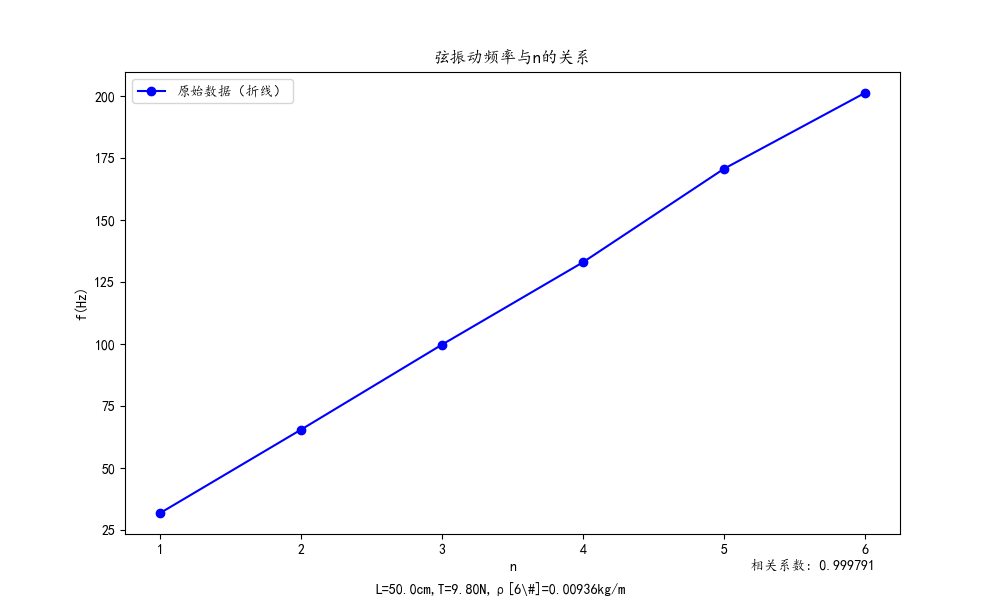
\includegraphics[scale=0.5]{1_original.png}
    \caption{弦振动频率与n的关系的原始数据}
    \label{29ea3b43}
\end{figure}


我们可以得到拟合结果如下图所示。
\begin{figure}[h]
    \centering
    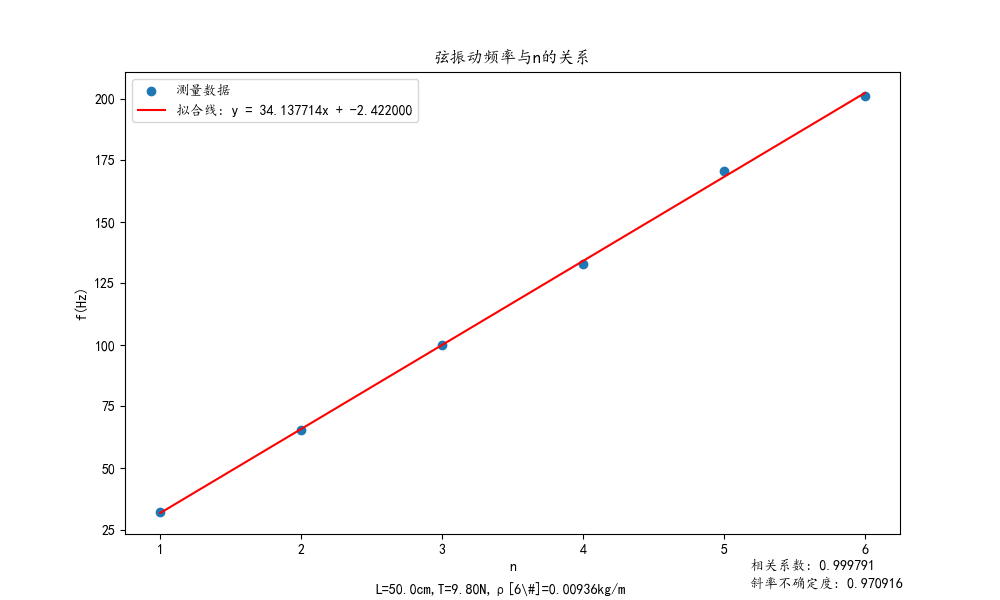
\includegraphics[scale=0.5]{1.png}
    \caption{弦振动频率与n的关系的拟合结果}
    \label{a709445a}
\end{figure}


由图可知,拟合结果为\ref{a709445a}:$y=34.137714x+-2.422000$。
\textbf{相关系数}为: 0.999791。
根据斜率不确定度的计算公式:
\begin{align}
    \Delta_{slope} & =t(N-2)\cdot S_{slope} \\ & = t(N-2)\cdot slope\cdot  \sqrt{\frac{\frac{1}{r^2}-1}{N-2}}\\ & = t(4)\cdot 34.13771428571428\cdot \sqrt{\frac{\frac{1}{0.9997907340439437^2-1}}{6-2}} \\ &= 0.970916
\end{align}